\chapter{Methodologies}

\label{chapter:methodologies}

\section{Facebook Multilingual Task Oriented Dialog}

\citet{schuster-etal-2019-cross-lingual} originally released the Facebook Multilingual Task Oriented Dialog (FMTOD) data set to encourage research in cross-lingual transfer learning for Natural Language Understanding (NLU) tasks; specifically from from high-resource to low-resource languages. The authors released the FMTOD data set with English as the high-resource language providing $\sim$43k annotated utterances, and Spanish and Thai as low-resource languages providing a total of $\sim$14k utterances. Furthermore, they streamlined the data set on two key tasks; namely intent detection and textual slot filling. In this thesis, we focus solely on the English language intent detection task in the FMTOD data set. This intent detection task entails a multi-label sequence classification task with a total of 12 classes from alarm, reminder and weather-related domains.

\subsection{Motivation}

We chose to work with the FMTOD data set since it is both a recently released and well-studied data set \citep{schuster-etal-2019-cross-lingual,zhang2019joint,zhang-etal-2020-intent}. We focus on the English language intent classification task since it is a relatively straightforward task which allows us to place a greater focus on performance and explainability. Furthermore, the English language subset entails the highest resources in the FMTOD data set. Finally, we find the FMTOD data set's intent detection classification especially attractive because it allows us to test the SoPa++ model on a multi-class NLU problem; which is significantly different from the focus on binary classification sentiment detection tasks in SoPa \citep{schwartz2018sopa}.

\subsection{Preprocessing}

We enumerate our preprocessing steps below:

\begin{enumerate}{}
  \item Similar to \citet{schwartz2018sopa}, we convert all FMTOD text samples to a lowercased format. This assists in simplifying the data set further.
  \item Next, we search through the pre-provided training, validation and test data partitions to remove duplicates within each partition.
  \item Finally, we remove data duplicates which overlap between partitions. During this step, we do not remove any cross-partition duplicates from the test partition in order to keep it as similar as possible to the original test partition. This comes into importance later when we compare performance evaluations on the test set with other studies.
\end{enumerate}

Many of the duplicates observed were already present in the original FMTOD data set, with additional duplicates being created from the initial lowercasing step. After preprocessing, we obtain a lowercased variant of the FMTOD data set with strictly unique data partitions. In the next section, we describe the summary statistics of the preprocessed FMTOD data set.

\begin{figure}[t]
  \centering
  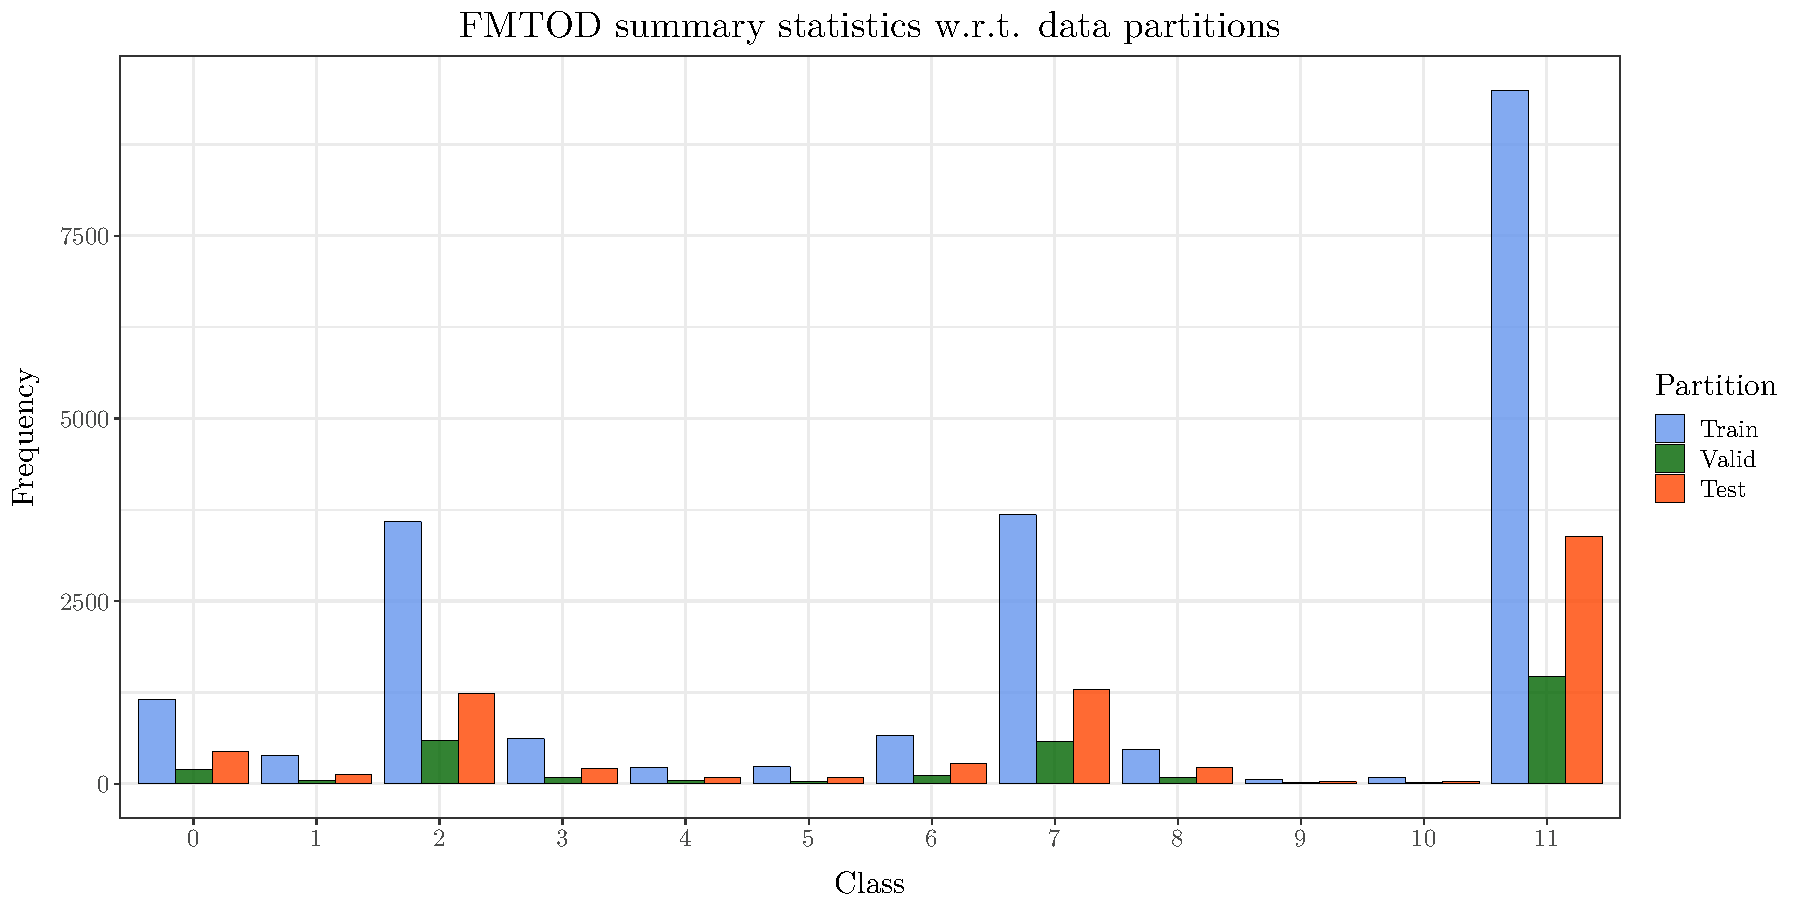
\includegraphics[width=14cm]{pdfs/generated/fmtod_summary_statistics.pdf}
  \caption{Data distribution of the preprocessed FMTOD data set grouped by classes and partitions}
  \label{fig:fmtod}
\end{figure}

\begin{table}[t!]
  \centering
  \begin{tabular}{lllll}
    \toprule
    Class and description & Train & Validation & Test & $\Sigma$ \\
    \midrule
    0: \texttt{alarm/cancel\_alarm} & 1157 & 190 & 444 & 1791 \\
    1: \texttt{alarm/modify\_alarm} & 393 & 51 & 122 & 566 \\
    2: \texttt{alarm/set\_alarm} & 3584 & 596 & 1236 & 5416 \\
    3: \texttt{alarm/show\_alarms} & 619 & 83 & 212 & 914 \\
    4: \texttt{alarm/snooze\_alarm} & 228 & 49 & 89 & 366 \\
    5: \texttt{alarm/time\_left\_on\_alarm} & 233 & 30 & 81 & 344 \\
    6: \texttt{reminder/cancel\_reminder} & 662 & 114 & 284 & 1060 \\
    7: \texttt{reminder/set\_reminder} & 3681 & 581 & 1287 & 5549 \\
    8: \texttt{reminder/show\_reminders} & 474 & 82 & 217 & 773 \\
    9: \texttt{weather/check\_sunrise} & 63 & 13 & 25 & 101 \\
    10: \texttt{weather/check\_sunset} & 88 & 11 & 37 & 136 \\
    11: \texttt{weather/find} & 9490 & 1462 & 3386 & 14338 \\[5pt]
    \hline \hline \\[-10pt]
    $\Sigma$ & 20672 & 3262 & 7420 & 31354 \\
    \bottomrule
  \end{tabular}
  \caption{Frequency of the preprocessed FMTOD data set classes grouped by partitions; $\Sigma$ signifies the cumulative frequency statistic}
  \label{tab:fmtod}
\end{table}

\subsection{Summary statistics}

Figure \ref{fig:fmtod} shows the summary statistics of the preprocessed FMTOD data set grouped by classes and data set partitions. Similarly, Table \ref{tab:fmtod} shows the same summary statistics in a tabular form with explicit frequencies. Based on the summary statistics, we can observe that the preprocessed FMTOD data set is significantly imbalanced with $\sim$45$\%$ of samples falling into Class 11 alone. We take this observation into consideration in later sections and apply fixes to mitigate this data imbalance. In addition, we observe from Table \ref{tab:fmtod-examples} that input utterances in the preprocessed FMTOD data set are generally short; with a mean input utterance length of 7.7 and a standard deviation of 2.5 tokens. Utterance length summary statistics were computed with the assistance of NLTK's default \texttt{Treebank} word tokenizer \citep{bird-loper-2004-nltk}.

\begin{table}[t!]
  \centering
  \begin{threeparttable}
  \begin{tabular}{lll}
    \toprule
    Class and description & Utterance length$^{\dagger}$ & Example$^{\ddagger}$ \\
    \midrule
    0: \texttt{alarm/cancel\_alarm} & 5.6 $\pm$ 1.9 & cancel weekly alarm \\
    1: \texttt{alarm/modify\_alarm} & 7.1 $\pm$ 2.5 & change alarm time \\
    2: \texttt{alarm/set\_alarm} & 7.5 $\pm$ 2.5 & please set the new alarm \\
    3: \texttt{alarm/show\_alarms} & 6.9 $\pm$ 2.2 & check my alarms. \\
    4: \texttt{alarm/snooze\_alarm} & 6.1 $\pm$ 2.1 & pause alarm please \\
    5: \texttt{alarm/time\_left\_on\_alarm} & 8.6 $\pm$ 2.1  & minutes left on my alarm \\
    6: \texttt{reminder/cancel\_reminder} & 6.6 $\pm$ 2.2 & clear all reminders. \\
    7: \texttt{reminder/set\_reminder} & 8.9 $\pm$ 2.5 & birthday reminders \\
    8: \texttt{reminder/show\_reminders} & 6.8 $\pm$ 2.2 & list all reminders \\
    9: \texttt{weather/check\_sunrise} & 6.7 $\pm$ 1.7 & when is sunrise \\
    10: \texttt{weather/check\_sunset} & 6.7 $\pm$ 1.7 & when is dusk \\
    11: \texttt{weather/find} & 7.8 $\pm$ 2.3 & jacket needed? \\[5pt]
    \hline \hline \\[-10pt]
    $\mu$ & 7.7 $\pm$ 2.5 & \textemdash \\
    \bottomrule
  \end{tabular}
  \begin{tablenotes}[flushleft]
    \footnotesize
    \item $^{\dagger}$Summary statistics follow the mean $\pm$ standard-deviation format
    \item $^{\ddagger}$Short and simple examples were chosen for brevity and formatting purposes
  \end{tablenotes}
  \end{threeparttable}
  \caption{Tabular summary of utterance length statistics and examples for FMTOD data classes; $\mu$ signifies the cumulative summary statistics}
  \label{tab:fmtod-examples}
\end{table}

\begin{table}[t!]
  \centering
  \def\arraystretch{1.3}
  \begin{tabular}{L{0.27\linewidth} L{0.45\linewidth} l}
    \toprule
    Study & Summary & Accuracy \\
    \midrule
    \citet{schuster-etal-2019-cross-lingual} & BiLSTM jointly trained on both the slot filling and intent detection English language tasks & 99.1$\%$ \\
    \citet{zhang2019joint} & BERT along with various decoders jointly fine-tuned on both the slot filling and intent detection English language tasks & 96.6--98.9$\%$ \\
    \citet{zhang-etal-2020-intent} & RoBERTa and XLM-RoBERTa fine-tuned on the English language and multilingual intent detection tasks respectively along with WikiHow pre-training & 99.3--99.5$\%$ \\
    \bottomrule
  \end{tabular}
  \caption{Tabular summary of studies that addressed the FMTOD intent detection English language task, along with their relevant summaries and accuracy range(s)}
  \label{tab:fmtod-results}
\end{table}

\subsection{Performance range}

Several studies have optimized deep learning models on the FMTOD English language intent classification task using a variety of models from BiLSTMs to XLM-RoBERTa \citep{schuster-etal-2019-cross-lingual,zhang2019joint,zhang-etal-2020-intent}. Table \ref{tab:fmtod-results} summarizes these studies along with their reported accuracy scores on the FMTOD English language intent classification task. Based on the presented results from these recent studies, we can infer that the general competitive accuracy range for the FMTOD English language intent classification task is from 96.6$\%$ to 99.5$\%$.

%%% Local Variables: 
%%% mode: latex
%%% TeX-master: "main"
%%% End: 